Another approach, referred to as \textit{cut-and-count} analysis,
 uses only the number of events selected with a reconstructed Higgs mass in the 
window $[\MH -6\%, \MH+10\%]$. The Higgs cross section limit is determined from the expected number of signal
and background events passing the selections $s$ and $b$ respectively.
%Lower Figure~\ref{fig:limit5fb} shows the same observed  limit on the ratio for the unblinded dataset, using the cut-and-count technique.
%The expectation for the full dataset is also shown in Figure~\ref{fig:limit5fb}~(down).
The results shown in Figure~\ref{fig:cutcount} are compatible with the full results.

\begin{figure}[htbp]
 \begin{center}
 \centerline{
 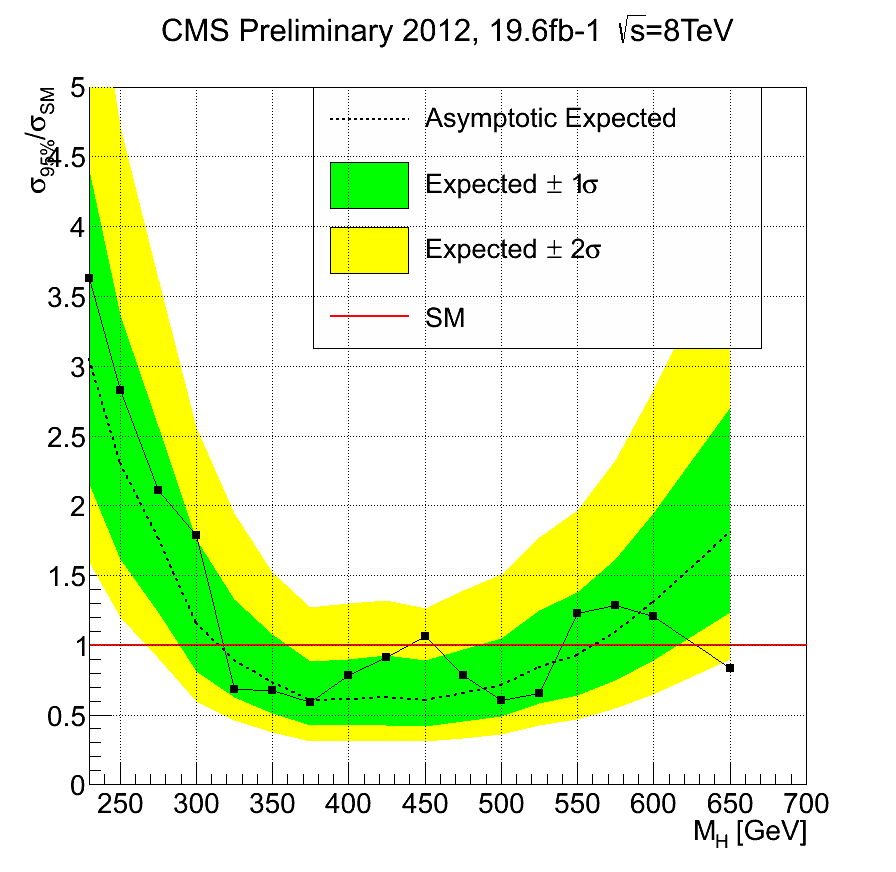
\includegraphics[width=0.49\textwidth]{plots/limit_CiC_unblinded_win0.png}
%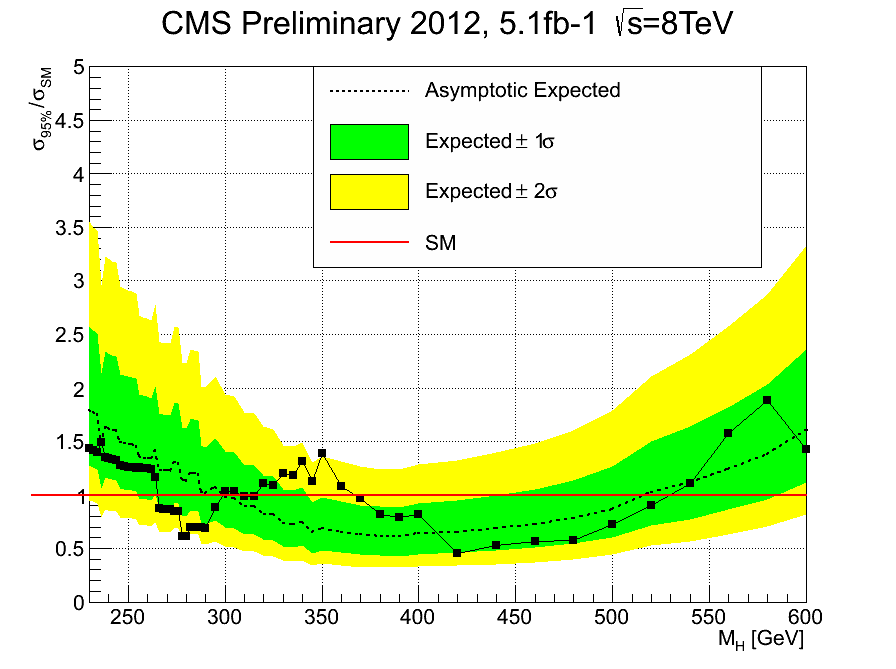
\includegraphics[width=0.49\textwidth]{plots/limit_CiC5_5fb_unblinded.png}
}
\caption{
Observed (solid) and expected (dashed) 95\% CL upper limit
on the ratio of the production cross section to the SM expectation
for the Higgs boson obtained using the \textit{cut-and-count} technique,
which integrates the mass distributions in a
range $[\MH -6\%, \MH+10\%]$ around each Higgs mass hypothesis.
The 68\% and 95\% ranges of expectation
for the background-only model are also shown with green and
yellow bands, respectively.  The solid line at 1 indicates the expectation
for a SM-Higgs-like boson.
}
\label{fig:cutcount}
\end{center}
\end{figure}
